\section{Hauptachsentransformation}

Sei $V$ ein euklidischer bzw. unitärer Vektorraum und $s$ eine hermitesche Sesquilinearform auf $V$.

\begin{proposition}
	\proplbl{6_7_1}
	Zu $A\in\Mat_n(K)$ hermitesch gibt es $S\in\Uni_n(K)$ so, dass
	\begin{align}
		S^*AS=S^{-1}AS=\diag(\lambda_1,...,\lambda_n)\notag
	\end{align}
	mit $\lambda_1,...,\lambda_n\in\real$.
\end{proposition}
\begin{proof}
	Da $A$ hermitesch ist, ist $f_A\in\End_K(K^n)$ selbstadjungiert, es gibt also nach \propref{6_6_5} also eine Orthonormalbasis $B=(x_1,...,x_n)$ aus Eigenvektoren von $f_A$. Die Transformationsmatrix $S=T^B_{\mathcal{E}}$ hat $x_1,...,x_n$ als Spalten und ist somit nach \propref{6_5_8} unitär. Nach \propref{6_6_3} sind die Eigenvektoren $\lambda_1,...,\lambda_n$ reell.
\end{proof}

\begin{conclusion}
	Sei $A\in\Mat_n(K)$ hermitesch. Genau dann ist $A$ positiv definit, wenn alle Eigenwerte positiv sind.
\end{conclusion}
\begin{proof}
	Nach \propref{6_7_1} existiert $S\in\Uni_n(K)$ mit 
	\begin{align}
	S^*AS=S^{-1}AS=D=\diag(\lambda_1,...,\lambda_n)\quad \lambda_1,...,\lambda_n\in\real\notag
	\end{align}
	Die Eigenwerte von $A$ sind die Eigenwerte von $S^{-1}AS$
	, also $\lambda_1,...,\lambda_n$. Sei $T=\overline{S}$. Genau dann ist $A$ positiv definit, wenn $T^tA\overline{T}=S^*AS=D$ positiv definit ist (\propref{6_2_8}), also wenn $\lambda_i>0$.
\end{proof}

\begin{theorem}[Hauptachsentransformation]
	Zu jeder hermiteschen Sesquilinearform $s$ auf $V$ gibt es eine Orthonormalbasis $B$ von $V$, für die 
	\begin{align}
		M_B(s)=\diag(\lambda_1,...,\lambda_n)\quad\lambda_1,...,\lambda_n\in\real\notag
	\end{align}
\end{theorem}
\begin{proof}
	Sei $B_0=(x_1,...,x_n)$ eine Orthonormalbasis von $V$ und $A=M_{B_0}(s)$. Da $s$ hermitesch ist, ist auch $A$ hermitesch (\propref{6_2_13}). Nach \propref{6_7_1} gibt es deshalb $S\in\Uni_n(K)$ mit $S^*AS=D$ eine reelle Diagonalmatrix. Ist nun $f\in\End_K(V)$ mit $M_{B_0}(f)=\overline{S}$, so ist auch $B=(f(x_1),...,f(x_n))$ eine Basis von $V$ mit $T^B_{B_0}=\overline{S}$ unitär. Da $M_{B_0}(f)$ unitär ist, ist auch $f$ unitär. Nach \propref{6_5_2} ist $f(B_0)=B$ somit auch eine Orthonormalbasis. Nach \propref{6_2_8} ist 
	\begin{align}
		M_B(s)=(T^B_{B_0})^t\cdot M_{B_0}(s)\cdot \overline{T^B_{B_0}}=S^*AS=D\notag
	\end{align}
\end{proof}

\begin{example}
	%TODO: mehr Abstand
	$A=\begin{henrysmatrix}2&1\\1&2\end{henrysmatrix}$, $s=s_A$, $K=\real$, $V=\real^2$ \\
	$\Rightarrow q_s(x)=2x_1^2+2x_1x_2+2x_2^2$ \\
	Wie verhält sich $q_s:\real^2\to\real$? Wie sehen die "'Höhenlinien"'
	\begin{align}
		H_c=\{x\in\real^2\mid q_s(x)=c\}\quad c\in\real\notag
	\end{align}
	aus?
	\begin{align}
		\chi_A=(t-2)^2-1=(t-1)(t-3)&\Rightarrow \lambda_1=3,\lambda_2=1\notag \\
		&\Rightarrow B=\left( \frac{1}{\sqrt{2}}\begin{henrysmatrix}1\\1\end{henrysmatrix},\frac{1}{\sqrt{2}}\begin{henrysmatrix}-1\\1\end{henrysmatrix}\right)\notag \\
		&\Rightarrow M_B(s)=\diag(3,1)\notag
	\end{align}
	Im neuen Koordinatensystem $z=\Phi_B^{-1}(x)$ ist dann
	\begin{align}
		q_s(z)=3z_1^2+z_2^2\notag
	\end{align}
	Mit $a_1=\frac{1}{\sqrt{3}}$, $a_2=1$ erhält man "'Höhenlinien"' der Form
	\begin{align}
		\left(\frac{z_1}{a_1}\right)^2+\left( \frac{z_2}{a_2}\right)^2=c\notag
	\end{align}
	was für $c>0$ eine Ellipse beschreibt.
	\begin{center}
		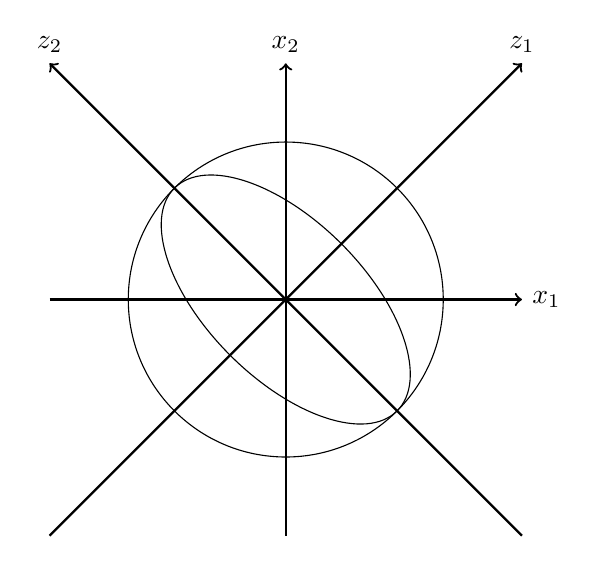
\begin{tikzpicture}
			\draw[->,thick] (-3,0) -- (3,0) node[right] {$x_1$};
			\draw[->,thick] (0,-3) -- (0,3) node[above] {$x_2$};
			\draw[rotate=-45] (0,0) ellipse (2cm and 1cm);
			\draw (0,0) circle (2);
			\draw[->,thick] (-3,-3) -- (3,3) node[above] {$z_1$};
			\draw[->,thick] (3,-3) -- (-3,3) node[above] {$z_2$};
		\end{tikzpicture}
	\end{center}
\end{example}

\begin{conclusion}
	\proplbl{6_7_5}
	Zu jeder hermiteschen Sesquilinearform $s$ auf $V$ gibt es eine Basis $B$ von $V$, für die 
	\begin{align}
		M_B(s)=\begin{pmatrix}\mathbbm{1_{r_{+}(s)}}&\;&\;\\\;&-\mathbbm{1_{r_{-}(s)}}&\;\\\;&\;&0\end{pmatrix}\notag
	\end{align}
	mit $r_+(s)+r_-(s)\le n$.
\end{conclusion}
\begin{proof}
	Sei $B_0=(x_1,...,x_n)$ eine Orthonormalbasis von $V$ mit $A=M_{B_0}(s)=\diag(\lambda_1,...,\lambda_n)$. Setze 
	\begin{align}
		\mu_i=
		\begin{cases}
			\frac{1}{\sqrt{\vert\lambda_i\vert}} & \lambda_i\neq 0 \\
			1 & \lambda_i=0
		\end{cases}\notag
	\end{align}
	Sei $x_i'=\mu_i\cdot x_i$ und $B'=(x'_1,...,x'_n)$. Dann ist $M_B(s)=S^tA\overline{S}$ mit $S=T^{B'}_{B_0}=\diag(\mu_1,...,\mu_n)$ also $M_{B'}(s)=\diag(\lambda'_1,...,\lambda'_n)$ mit $\lambda'_i=\mu_i\cdot \lambda_i\cdot\overline{\mu_i}=\mu_i^2\lambda_i\in\{0,1,-1\}$. Durch Permutation der Elemente von $B'$ erhält man die gewünschte Basis $B$.
\end{proof}

\begin{definition}[Ausartungsraum]
	Der \begriff{Ausartungsraum} von $s$ ist
	\begin{align}
		V_0=\{x\in V\mid s(x,y)=0\quad\forall y\in V\}\notag
	\end{align}
\end{definition}

\begin{lemma}
	$V_0$ ist ein Untervektorraum von $V$.
\end{lemma}
\begin{proof}
	Klar aus Linearität im ersten Argument.
\end{proof}

\begin{lemma}
	\proplbl{6_7_8}
	Seien $V_+$ und $V_-$ Untervektorräume von $V$ mit $V=V_+\oplus V_-\oplus V_0$ und $s$ positiv definit auf $V_+$, $-s$ positiv definit auf $V_-$. Dann ist
	\begin{align}
		\dim_K(V_+)&=\max\{\dim_K(W)\mid \text{Untervektorraum von }V,s\text{ positiv definit auf }V\}\notag \\
		\dim_K(V_-)&=\max\{\dim_K(W)\mid \text{Untervektorraum von }V,-s\text{ positiv definit auf }V\}\notag
	\end{align}
\end{lemma}
\begin{proof}
	Beweis nur für $V_+$, analog für $V_-$. \\
	$\le$: klar \\
	$\ge$: Ist $W\le V$ Untervektorraum mit $s(x,x)>0\quad\forall x\in W\backslash\{0\}$, so ist $W\cap(V_-\oplus V_+)=\{0\}$. Ist $x=y+z$ mit $y\in V_-$, $z\in V_0$, so ist $s(x,x)=s(y+z,y+z)=\underbrace{s(y,y)}_{\le 0}+\underbrace{s(y,z)+s(z,y)+s(z,z)}_{=0}\le 0\Rightarrow \dim_K(W)\le \dim_K(V)-\dim_K(V_-)-\dim_K(V_0)=\dim_K(V_+)$.
\end{proof}

\begin{theorem}[Trägheitssatz von \person{Sylvester}]
	Für eine hermitesche Sesquilinearform $s$ auf $V$ sind die Zahlen $r_+(s)$, $r_-(s)$ aus \propref{6_7_5} eindeutig bestimmt.
\end{theorem}
\begin{proof}
	Sei $B$ eine Basis von $V$ wie in \propref{6_7_5}, $B=(x_1,...,x_n)$. Definiere
	\begin{align}
		V_+&=\Span_K(x_1,...,x_{r_+(s)})\notag \\
		V_-&=\Span_K(x_{r_+(s)+1},...,x_{r_+(s)+r_-(s)})\notag \\
		V'_0&=\Span_K(x_{r_+(s)+r_-(s)+1},...,x_n)\notag
	\end{align}
	Dann ist $s$ positiv definit auf $V_+$, $-s$ positiv definit auf $V_-$ und $V=V_+\oplus V_-\oplus V'_0$. Es gilt $V'_0=V_0$\\
	$\subseteq$: klar \\
	$\supseteq$: Ist $x=\sum_{i=1}^{n} \lambda_ix_i\in V_0$, so ist $0=s(x,x_i)=\lambda_i\cdot s(x_i,x_i)$ für $i=1,...,n$ also $\lambda_i=0$ für $i=1,...,r_+(s)+r_-(s)$, d.h. $x\in V'_0$. Nach \propref{6_7_8} ist $r_+(s)=\dim_K(V_+)$ nur von $s$ abhängig, analog für $r_-(s)$.
\end{proof}

\begin{definition}[Signatur]
	Die \begriff{Signatur} von $s$ ist das Tripel
	\begin{align}
		(r_+(s),r_-(s),r_0(s))\notag
	\end{align}
	wobei $r_0(s)=\dim_K(V_0)$.
\end{definition}

\begin{conclusion}
	Ist $s$ eine hermitesche Form auf $V$ und $B$ eine Basis von $V$, so ist die Zahl der positiven bzw. negativen Eigenwerte von $M_B(s)$ gleich $r_+(s)$ bzw. $r_-(s)$, insbesondere also unabhängig von $B$.
\end{conclusion}
\begin{proof}
	Sei $A=M_B(s)$. Nach \propref{6_7_1} gibt es $S\in\Uni_n(K)$ mit $S^*AS$ eine reelle Diagonalmatrix. Da $S^*=S^{-1}$ haben $A$ und $S^*AS$ die selben Eigenwerte. Bringt man $S^*AS$ nun in die Form in \propref{6_7_5}, so ändern sich die Vorzeichen der Diagonale nicht mehr.
\end{proof}